\documentclass{standalone}
\usepackage{tikz}
\usetikzlibrary{calc, intersections}

\begin{document}
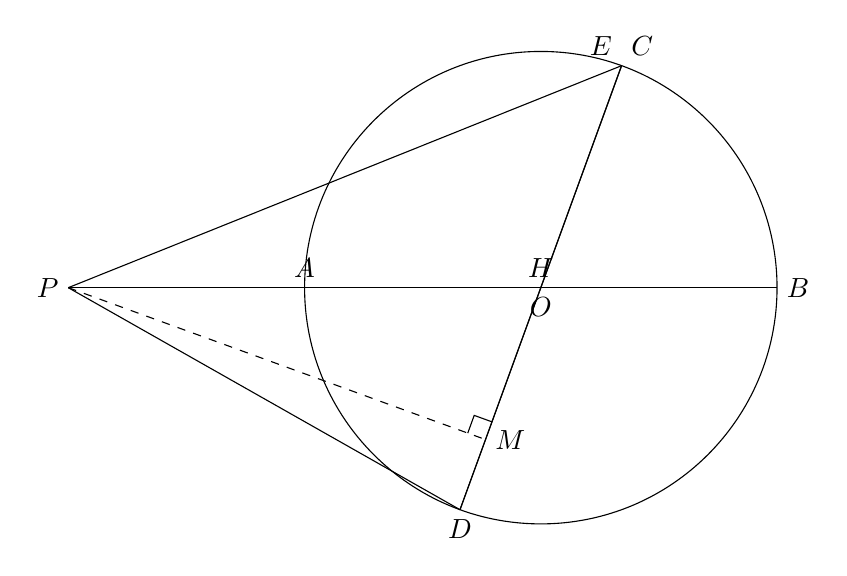
\begin{tikzpicture}[scale=1.2]
    % Define coordinates
    \coordinate (O) at (0,0);
    \coordinate (P) at (-5,0);
    
    % Circle
    \draw (O) circle (2.5cm);
    
    % Points on the horizontal line
    \coordinate (A) at (-2.5, 0);
    \coordinate (B) at (2.5, 0);
    
    % Point C (angle 70 degrees)
    \coordinate (C) at (70:2.5);
    
    % Point D (opposite to C, so CD is diameter)
    \coordinate (D) at (250:2.5);
    
    % Line PC intersects circle at E and C
    \path[name path=linePC] (P) -- (C);
    \path[name path=circle] (O) circle (2.5);
    \path [name intersections={of=linePC and circle, by={E, C_calc}}];
    
    % Line ED intersects AB at M_pos
    \path[name path=lineED] (E) -- (D);
    \path[name path=lineAB] (A) -- (B);
    \path [name intersections={of=lineED and lineAB, by={M_pos}}];
    
    % Point H_pos is projection of P onto OD
    \coordinate (H_pos) at ($(O)!(P)!(D)$);
    
    % Draw lines
    \draw (P) -- (B); % Line PAB
    \draw (P) -- (C); % Line PEC
    \draw (C) -- (D); % Diameter CD
    \draw (E) -- (D); % Chord ED
    \draw (P) -- (D); % Line PD
    \draw[dashed] (P) -- (H_pos); % Altitude PH
    
    % Right angle mark at H_pos
    \coordinate (X) at ($(H_pos)!2mm!(P)$);
    \coordinate (Y) at ($(H_pos)!2mm!(O)$);
    \draw (X) -- ($(X)+(Y)-(H_pos)$) -- (Y);
    
    % Labels (Swapped M and H as per instruction)
    \node[left] at (P) {$P$};
    \node[above] at (A) {$A$};
    \node[above] at (M_pos) {$H$}; % Originally M, now H
    \node[below] at (O) {$O$};
    \node[right] at (B) {$B$};
    
    \node[above left] at (E) {$E$};
    \node[above right] at (C) {$C$};
    \node[below] at (D) {$D$};
    \node[right] at (H_pos) {$M$}; % Originally H, now M
    
\end{tikzpicture}
\end{document}
